\chapter{Design}
\label{ch:design}

% In this chapter, we describe the overall design of our solution to the problem identified in \Cref{ch:introduction}, building on work described in \Cref{ch:background}.
% Figure~\ref{fig:topview} shows the top view of the project with modules interconnected.
% \begin{figure*}[t!]
% \begin{figure*}[h]
% \centering
%   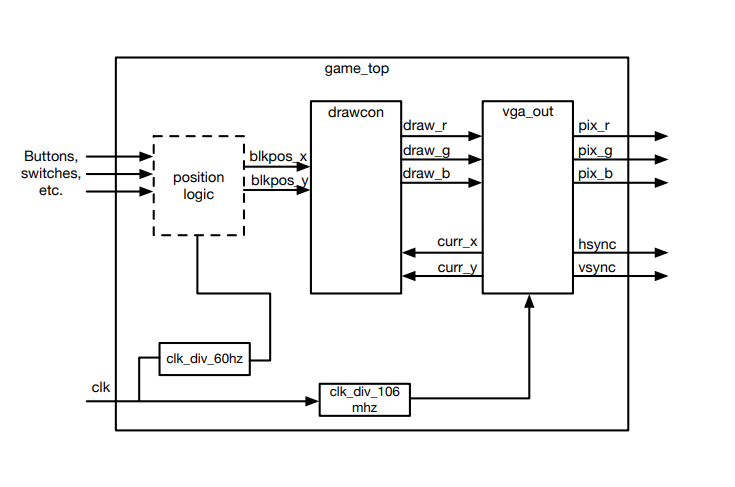
\includegraphics[width=0.8\textwidth,keepaspectratio]{../figures/modules overview.png}
%   \caption{Block diagram of the proposed triple-core lockstep technique (TCLS)}
% \label{fig:topview}
% \end{figure*}

在程序设计上,通过将问题抽象,主要实现了以下几个class.

\begin{itemize}
  \item Function: 函数的接口类,要求实现operator()接口,即可以通过函数(参数)的形式来获得函数值
  \item BoundaryCondition: 代表边界条件的类,可以通过Type()获取某一点是Dirichlet条件还是Neumann条件,通过Value()获取相应函数值,这两个方法本质上都是某个Function的间接调用
  \item Cycle: 代表了定义域被减去的圆盘,其中有BoundaryCondition作为成员,并且可以判断一个点是否在圆盘上
  \item Domain: 代表了定义域,将BoundaryCondition和Cycleu作为成员,可以判断自身连通性
  \item Solver: 代表求解器,将Domain作为成员,实现有限差分法的求解.
\end{itemize}

此外,Tensor模板类代表了张量,Solver中的Matrix和Vector分别是其为二阶和一阶并且储存double值的情况.FunctionExtension则是
继承Function类的函数类的集合,最终求解器接受这些函数作为输入进行初始化.ExpressionTree中为表达树的实现,可以解析带有cmath函数和自变量的字符串并求值.
Assistance中为一些辅助函数.JsonRead中定义了读取jsona文件并接受所定义的函数进行Solver初始化,求解,输出的函数(误差的$max-norm,2-norm,1-norm$被依次打印在命令行中).